\documentclass{article}
\usepackage[utf8]{inputenc}
\usepackage{graphicx}
\usepackage{hyperref}
\title{Minando Datos y algortimos de clasificación.}
\author{Rodrigo Reyes M.}
\begin{document}
\maketitle

\section{Introducción a la minería de datos.}
La minería de datos es la intersección entre tres grandes Ciencias o Áreas de Conocimiento, la estadística, las ciencias computacionales y la matemática.
En el área de estadística los modelos y las teorías de eventos estocásticos son la herramienta principal para describir e inferir de un conjunto de datos, mientras que en ciencias computacionales las bases de datos y los algoritmos de inteligencia artificial son indispensables para guardar y \textit{minar o buscar patrones} en los datos.La matemática es el pegamento que une ambas ciencias y permite describir formalmente muchas de la teorías y modelos.

Actualmente existen una plétora de empresas privadas y gubernamentales alrededor del orbe con especialistas en obtener información no evidente de los datos que se obtienen o capturan.

Desde Facebook, que vende y utiliza información acerca de los hábitos de consumo y permite generar campañas de Marketing adecuadas a la demografía y el \textit{target audience}.

En el mundo el rápido desarrollo de las tecnologías de la información y las redes de comunicación permiten la generación de un alud de información cada segundo.

Gran parte de los descubrimientos respecto a los patrones de consumo se utilizan para mejorar la toma de decisiones.Respaldando con datos duros para disminuir el riesgo de una decisión mal tomada.



\subsection{Clasificar un conjunto de datos}
Existen miles de algoritmos que clasifican datos, algunos utilizan cómputo distribuido, o bien se respaldan de algoritmos genéticos y de redes bayesianas.

En el curso se verán tres algoritmos básicos, haciendo mención de algoritmos más avanzados.Los algoritmos básicos de clasificación son:
\begin{enumerate}
\item K-NN (K Nearest Neighbor)
\item Regresión Lineal
\item K-means
\end{enumerate}
\subsection{Atributos de los datos}
Algo muy importante de considerar al clasificar datos es determinar si son \textit{separable linealmente} es decir que mediante una línea recta podemos separar el espacio y clasificar los datos correctamente, los datos \textit{separables no-linealmente} son aquellos que mediante una línea no recta (o círculo) se pueden separar.También existen datos \textit{inseparables} que son aquellos que no se pueden separar de ninguna manera.
\begin{figure}[h]
\centering
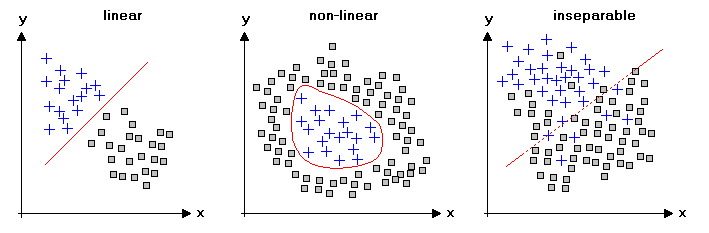
\includegraphics[width=10cm, height=4cm]{hl_classif_separation.png}
\caption{Distintos tipos de separabilidad}
\label{fig:my_label}
\end{figure}
\subsection{Traducción de datos}
Generalmente para que funcionen correctamente los algoritmos es necesario convertir los datos a un nivel de abstracción más alto, un dato que se encuentra a ese nivel se le denomina \textit{feature}.
Por ejemplo, supongamos que tenemos una serie de datos sobre un grupo de personas edad, peso y nacionalidad.En el caso de la edad generalmente se representa mediante un entero que define la cantidad de años de vida de la persona, así pues el número 25 al ser una representación numérica de la edad de una persona se le considera un \textit{feature}.Similarmente el peso generalmente se mide en kilogramos, sin embargo nótese que el nivel de precisión debe ser estándar, es decir si se desea representar los pesos con diversas precisiones decimales deben ser las mismas para todos los datos para poder ser un \textit{feature}.Ahora la nacionalidad puede ser representada mediante un número que corresponda a el índice de una lista de países, es decir \textit{mapeamos} el país a un número entero de un rango acotado.Lo más importante de la traducción es evitar que se pierda información que distingue a cada uno de los componentes de un vector de datos. Por ejemplo,si al traducir la nacionalidad decidimos no mapear a Groelandia y traducir a los nacidos en Groelandia como nacionalidad danesa destriumos ésa parte de la información y al agrupar el conjunto por ejemplo por continente, consideramos a los groelandeses como parte del contiente europeo.A pesar que geográficamente está considerado parte de el continente Americano.Evitar la pérdida de información depende del uso que se desea dar y de la importancia de algunos atributos.Igualmente en general se desea reducir lo más posible la dimensionalidad de los datos, es decir la cantidad de \textit{features} con las que se representan los puntos.(Se puede decir que la cantidad de campos en un registro de una base de datos equivale a su dimensionalidad)
\subsection{Ejercicios}
\begin{enumerate}
\item Transforma los datos en \verb#usuarios_banco.csv# a su forma de vectores de \textit{features} y guardalo como \verb#usuarios_banco_traducidos.csv# serán utilizados en otros ejercicios.
Tips:Recuerda que los datos que no son numéricos ya sea que se mappen a un valor numérico ó se descarten por no ser relevantes.Piensa ¿Qué datos son necesarios y cuáles no?
\item Explica, ¿Cómo fue la traducción de cada uno de los componentes?
\end{enumerate}

\section{K-NN (K-Nearest Neighbor)}
El algoritmo K-NN o el k-ésimo vecino más cercano es un algoritmo de clasificación \textit{supervisado}.Es decir que permite clasificar puntos utilizando clasificaciones previas, comúnmente llamadas conjunto de entrenamiento ó \textit{training set}.Por ejemplo supongamos que queremos saber el idioma de un texto basado en la frecuencia de la letra 't'. El archivo \verb#clasificados_textos.csv# contiene 40 frecuencias de la letra 't' en tres idiomas distintos: Inglés,Español y Alemán.(1,2,3 respectivamente)
Aquí una gráfica con los puntos graficados con distintos colores dependiendo de el idioma del cual fueron escritos.\autoref{fig:fig2}
La primer coordenada corresponde a la cantidad de letras en total y la segunda coordenada corresponde a el porcentaje del total que representa la letra 't' en el texto.


\begin{figure}[h]
\centering
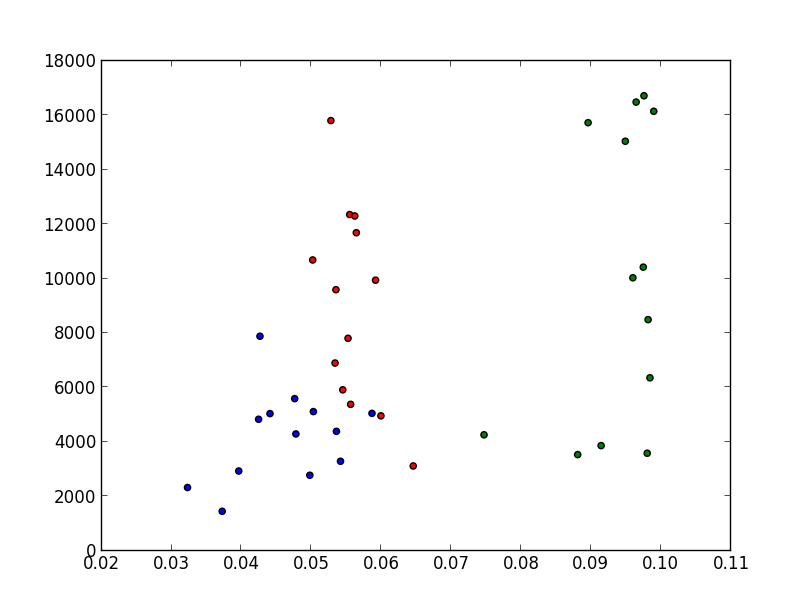
\includegraphics[width=10cm, height=8cm]{idiomas.png}
\caption{Frecuencia de la letra 't' en tres idiomas distintos }

\label{fig:fig2}
\end{figure}
Ahora supongamos que queremos catalogar el siguiente punto:

\verb#(8450, 0.09372781065088757)# que se obtiene al obtener la cantidad de letras y la frecuencia de la letra 't' del archivo \verb#no_clasificado.txt#
Queremos catalogar con el idioma (Inglés,Alemán o Español)
Primero encontramos los elementos que están a una distancia de un radio k (se determina un vector unitario k=1 basándose muchas veces en la dispersión de los puntos en el espacio) tomando como centroide la coordenada que deseamos catalogar.
Luego se decide basándose en una especie de \textit{votación}, es decir de los puntos dentro de el radio ¿cuáles abundan más?
(Si empatan el algoritmo puede ya sea elegir al azar ó utilizar un segundo criterio como por ejemplo el punto más cercano a qué categoría corresponde)
En nuestro ejemplo podemos ver que los siguientes son los candidatos y que al ser más abundantes los puntos catalogados como Inglés (de hecho en éste ejemplo no hay puntos con otro idoma) se cataloga el texto como Inglés.
\begin{table}[h]
\centering
\begin{tabular}{c|c|c}
 No. de letras & Proporcion de letras 't' & Idioma \\
\hline
 6353 &   0.09837871871556744 & Inglés \\
 8490 & 0.09811542991755005 & Inglés \\
 10418 & 0.09742752927625264 & Inglés \\
\end{tabular}
\caption{Puntos cercanos al centroide}
\label{tab:my_label}
\end{table}


\subsection{Ejercicios}
\begin{enumerate}
\item Utilizando el archivo \verb#usuarios_banco_traducidos.csv#, gráfica dos dimensiones que crees son relevantes para admitir o aceptar una línea de crédito.
\item Define una línea que separe los aceptados de los rechazados.Crea un segundo archivo \verb#usuarios_banco_entrenamiento.csv# que contenga una columna extra, la columna si es 1 indica aceptado y si es 0 es rechazado.Procura cumplir con tu línea de separación.
\item Puedes realizar tanto a mano, como utilizando algún programa la clasificación de \verb#solicitud_credito.csv# y decidir si es o no aceptado según el algoritmo K-NN.
\end{enumerate}

\section{Regresión Lineal}

La regresión lineal no es por sí solo un algortimo, es un método matemático para encontrar la relación entre variables independientes y una variable dependiente.(Suponinedo que existe tal)
Es muy importante destacar que permite proyectar datos nuevos basándose en datos conocidos, además no funciona muy bien con dimensiones superiores a 3.Así pues no clasifica datos en agrupamientos, más bien acomoda de cierta forma el punto a proyectar sobre una línea que se traza a través de los datos.(Una función) Hay que tener especial cuidado al utilizar éste método debido a que hacemos varias suposiciones acerca de la naturaleza de los datos previos.(Que no son estocásticos y que presentan homoestacidad.)


Un algoritmo muy común para realizar regresión lineal es mediante mínimos cuadrados ó \textit{least squares}.
Se define como el mínimo del cuadrado de la suma de la diferencias entre el vector dependiente y los vectores independientes.Beta es aquel valor que nos permite ajustar la suma para que sea mínima (cercana a cero).
$$ argmin(\Sigma_i (y_i - \beta x_i)^2) $$
En Numpy existe el paquete de álgebra lineal que permite calcular el ajuste de mínimos cuadrados y la línea que define tal ajuste.
\verb#linalg.lstsq(A,B)# ésta función nos regresa las soluciones de el sistema de ecuaciones.
Es decir dado una matriz A de n x m y un vector b de dimensión m.
El vector (de dimensión n) que retorna satisface la siguiente ecuación.
$$ Ax = b $$




\section{K-means}
El algoritmo de K-means es un algortimo de clasificación \textit{no supervisado}, es decir no requiere de un conjunto de entrenamiento para poder definir un conjunto.En general éstos algoritmo se utilizan principalmente para descubrir datos parecidos ó cercanos (en el hiperplano).
Por ejemplo tenemos tres tipos distintos de países.
\begin{enumerate}
\item desarrollado
\item en vías de desarrollo
\item subdesarrollado
\end{enumerate}
Ahora con un vector de dos dimensiones:
Producto Interno Bruto (PIB) per cápita (que se obtiene dividiendo el PIB entre la población total en millones) y expectativa de vida
Tenemos los datos de 30 paises mezclados entre desarrollados, en vias de desarrollo y subdesarrollados.
\begin{figure}[h]
\centering
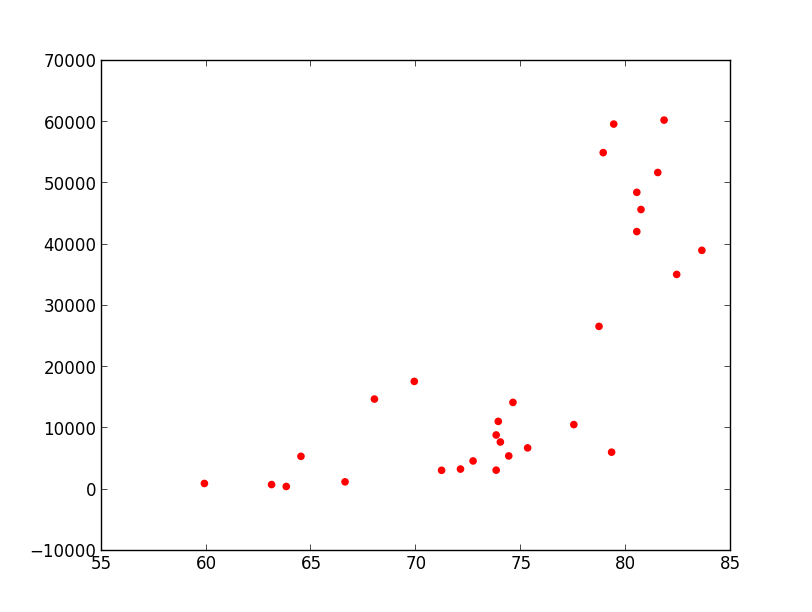
\includegraphics[width=10cm, height=8cm]{paises_plot1.png}
\caption{Expectativa de Vida vs PIB per cápita en 30 países}
\label{fig:fig}
\end{figure}

Ahora utilizando Numpy podemos utilizar una implementación del algoritmo de K-means.(Para saber más a detalle el funcionamiento de k-means se sugire el siguiente link) \url{http://www.bytemuse.com/post/k-means-clustering-visualization/}
Se utiliza importando las bibliotecas de clustering
\verb#from scipy.cluster.vq import vq, kmeans#.Una vez importada podemos utilizar la función \verb#kmeans(matriz,k)# que recibe una matriz de \textit{features} y las agrupa en k grupos.
Ésto nos regresa una matriz con k centroides y el nivel de distorsión entre los centroides y los datos.
Ahora podemos ver que los grupos quedan de la siguiente forma:

\begin{table}[h]
\centering
\begin{tabular}{c|c|c}
 Nombre del país & Grupo \\
\hline
México & grupo 1\\
Corea del Sur & grupo 1\\
Brasil & grupo 1\\
Venezuela & grupo 1\\
Rusia & grupo 1\\
Trinidad y Tobago & grupo 1\\
Guatemala & grupo 2\\
Nambia & grupo 2\\
Tonga & grupo 2\\
Micronesia & grupo 2\\
Corea del Norte & grupo 2\\
Zimbabue & grupo 2\\
Egipto & grupo 2\\
China & grupo 2\\
Cuba & grupo 2\\
Tailandia & grupo 2\\
Colombia & grupo 2\\
Haiti & grupo 2\\
Rumania & grupo 2\\
Pakistán & grupo 2\\
Estados Unidos de América & grupo 3\\
Alemania & grupo 3\\
Japón & grupo 3\\
Reino Unido & grupo 3\\
Canadá & grupo 3\\
Suecia & grupo 3\\
Dinamarca & grupo 3\\
Italia & grupo 3\\
Bélgica & grupo 3 \\
\end{tabular}
\caption{Agrupamiento de países utilizando kmeans}
\label{tab:my_label}
\end{table}
Es fácil ver que los grupos corresponden a lo siguiente
\begin{table}[h]
\centering
\begin{tabular}{c|c|c}
 grupo 1 & País en vias de desarrollo \\
\hline
 grupo 2 & País en subdesarrollado \\
\hline
 grupo 3 & País desarrollado \\
\hline

\end{tabular}
\caption{Mapeo de agrupamientos a tipos de paises}
\label{tab:my_label}
\end{table}

Es muy probable que algunos paises estén mal catalogados, sin embargo esto es muchas veces debido a la cercanía que hay entre paises de PIB per cápita y expectativa de vida similares.Sin embargo como se puede apreciar en la gráfica de puntos los países más ricos son bastante distinguibles entre el resto, por tanto el grupo de paises desarrollados es en general bien catalogado.Cabe destacar que el algoritmo no necesita ningún conjunto de entrenamiento, sin embargo al sólo arrojar grupos las etiquetas deben ser mapeadas manualmente.En el ejemplo se usó el \textit{know how} ó el conocimiento empírico para poder discernir éste mapeo.
\end{document}
